\documentclass{article}
\usepackage{fancyhdr}
\usepackage[utf8]{inputenc}
\usepackage{amssymb}
\usepackage{tabularx}
\usepackage{lmodern}
\usepackage{cite}
\usepackage{listings}
\usepackage{subfig}
\usepackage{algorithm2e}
\usepackage{color}
\usepackage{amsmath}
\setcounter{tocdepth}{3}
\usepackage{polski}
\usepackage{amssymb}
\newcommand*{\QEDA}{\hfill\ensuremath{\blacksquare}}%
\newcommand*{\QEDB}{\hfill\ensuremath{\square}}%<Paste>
\usepackage[a4paper]{geometry}
\usepackage{psfrag}
\usepackage{bbm}
\usepackage[T1]{fontenc}
\usepackage{color}
\usepackage{url}
\usepackage[dvipsnames]{xcolor}
\usepackage{float}
\usepackage{mathtools}
\usepackage{hyperref}
\usepackage{algorithmic}
\usepackage{psfrag}
\usepackage{graphicx}




\hypersetup{
    colorlinks=true,
    linkcolor=violet,
    filecolor=magenta,      
    citecolor=blue,
    urlcolor=violet,
}
\graphicspath{{graphics/}}
\DeclarePairedDelimiter\ceil{\lceil}{\rceil}
\DeclareMathOperator*{\argmin}{argmin}
\DeclarePairedDelimiter\floor{\lfloor}{\rfloor}
\DeclareGraphicsExtensions{.eps}
\DeclareGraphicsExtensions{.ps}




\newcommand{\wek}[1]{
	{\bf{#1}} 
}
\newcommand{\jed}[1]{
	{$\left[#1\right]$}
}
\newcommand{\mat}[1]{
	{\bf #1} 
}
\newcommand{\todo}[1]{
	\colorbox{yellow} {{\color{red}
	\emph {TODO: #1}
}}}
\newcommand{\srednia}[1]{
	\langle #1 \rangle 
}
\providecommand{\tightlist}{%
  \setlength{\itemsep}{0pt}\setlength{\parskip}{0pt}}



\pagestyle{fancy}

\def\lecturemark{}
\fancyhf{}
\fancyhead[L]{\lecturemark}
\fancyfoot[C]{\thepage}
\newcommand{\spr}[1]{\part{#1}\def\lecturemark{\partname\ \thepart: #1}}
\renewcommand{\partname}{Sprawozdanie}
\usepackage{etoolbox}% for \patchcmd
\renewcommand{\thepart}{\arabic{part}}
\makeatletter
\patchcmd{\@part}{\par\nobreak}{: }{}{}
\patchcmd{\@part}{\huge}{\Large}{}{}
\makeatother
\newcommand{\argmax}{\operatornamewithlimits{argmax}} 

\title{Systemy agentowe: \\ Wieloagentowy symulator rynku\\ Dokumentacja końcowa}
\author{Aleksandra Dzieniszewska \\ Jakub Łyskawa \\ Eryk Warchulski\\ Prowadzący: dr inż. Dominik Ryżko}%
\date{\today\\wer. 1.0}

\begin{document}

\maketitle
{\footnotesize{\tableofcontents}}
\topskip0pt
\vspace*{\fill}

\newpage
\section{Wprowadzenie}

Celem niejszego projektu była implementacja symulatora rynku dóbr konsumpcyjnych w oparciu o paradygmat systemów wieloagentowych. 
Dokument ten składa się z trzech sekcji: w sekcji (\ref{sec1}) omówiony jest model agenta oraz modelu rynku, którego dotyczą symulacje.
Sekcja (\ref{sec2}) zawiera opis architektury systemu, tj. modułów 
oraz sposobu ich działania, które składają się na system. Sekcja ostatnia -- (\ref{sec3}) -- zawiera opis przykładowych symulacji, które
można przeprowadzać w ramach dostarczonego systemu.

\section{Model zjawiska \label{sec1}}

Przedstawiony w tej sekcji model zjawiska jest spójny z dokumentacją wstępną.\footnote{Dokumentacja wstępna zamieszczona jest pod niniejszym \href{https://github.com/warbarbye/Multi-agent-market/blob/master/doc/dokumentacja-wstepna.pdf}{adresem}.} 

\subsection{Model rynku}
Rynek determinowany jest poprzez strukturę połączeń między agentami przy czym struktura połączeń jest generowana przez wybrany graf losowy
(Barabasi-Albert, dowolony inny lub zadany przez użytkownika). Rynek działa ciągle i po czasie $t$ jego stan jest archiwizowany, co jest niezależne od podmiotów-agentów na rynku.

\subsection{Model Agenta}
\subsubsection{Zasoby}
\begin{itemize}
\tightlist
\item
  agent \(A_i\) w chwili \(t\) posiada \(Z^{A_i}(t)\) zasobu i ma
  możliwość wygenerować większą jego ilość, która będzie go kosztowała
  \(g(z)\), gdzie \(z\) jest przyrostem zasobu
\item
  agent może przechowywać zasób lub go sprzedać, wchodząc w negocjacje
  handlowe z pozostałymi agentami na rynku, z którymi agent jest
  połączony (patrz struktura połączeń)
\item
  produkcja agenta jest ograniczona przez \(P^{A_i}_{max}(t, \delta t)\)
\item
  każdy agent posiada maksymalny stan magazynowy zasobu \(Z\), którego
  nie może przekroczyć, i wynosi on \(M^{A_i}\)
\item
  jeśli agent przekroczy maksymalny stan posiadania \(M^{A_i}\), to
  zobligowany jest do zapłacenia kosztu utylizacji nadmiarowej ilości
  zasobu \(Z\)
\item
  agenty mają potrzeby konsumpcyjne \(C^{A_i}(t, \delta t)\), które chcą
  zaspokoić
\item
  jeśli agent nie zaspokoi swoich potrzeb konsumpcyjnych po czasie \(T\)
  od ich wygenerowania, to zobligowany jest do zapłacenia kosztu
\item
  agenty posiadają na starcie określoną ilość środka wymiany
  \(K^{A_i}\), który jest im przydzialny w sposób losowy lub
  zdeterminowany przy inicjalizacji systemu
\item
  agent otrzymuje środek wymiany zgodnie z funkcją \(f^{A_i}(\dot)\)
\end{itemize}

\subsubsection{Polityka decyzyjna}

Polityka decyzyjna określa zachowanie agentów na rynku.

Przyjmuje się, że polityka decyzyjna agenta sparametryzowana jest
następującymi wielkościami:

\begin{itemize}
\tightlist
\item
  obecne zapotrzebowanie agenta \(R \geq 0\)
\item
  czas, w którym agent musi zaspokoić swoje zapotrzebowanie \(T_s\)
  liczony od czasu startu sesji
\item
  obecny stan agenta \(S\), który jest liczbą posiadanych jednostek
  zasobu \(Z\) przez agenta
\item
  obecny budżet agenta \(B\), który jest liczbą posiadanych jednostek
  wymiany \(K\) przez agenta
\item
  funkcją kosztu produkcji \(g(z)\)
\item
  funkcją limitu produkcji \(P(t, \delta t)\)
\item
  kosztem utylizacji dóbr nadmiarowych \(M_c\)
\item
  kosztem niezaspokojenia potrzeb konsumpcyjnych \(C\)
\item
  limitem posiadanych jednostek zasobu \(M\)
\end{itemize}

Agent w oknie czasowym \(T_w\), wyznaczającym czas trwania negocjacji,
generuje oferty sprzedaży (obiekt \texttt{Os}) oraz kupna (obiekt
\texttt{Ob}), na które nałożone są limity:

\begin{itemize}
\tightlist
\item
  \texttt{Ob.value} \(\leq B\) \(\land\) \texttt{Ob.n} \(\leq M - S\),
  które kolejno oznaczają: cena zakupionej ilości towaru nie może
  przekraczać budżetu agenta oraz ilość zakupionego towaru nie może być
  większa od dostępnej jeszcze liczby jednostek zasobu, które agent może
  przechowywać.\\
\item
  \texttt{Os.n} \(\leq S\), tj. ilość sprzedanego towaru nie może być
  większa pod stan posiadania agenta.
\end{itemize}

Na podstawie powyższych ustaleń proponowana polityka decyzyjna agenta
może być wyglądać następująco:

\begin{itemize}
\tightlist
\item
  \texttt{Os}, \texttt{Ob} są
  aktualnymi ofertami kupna i sprzedaży
\item
  \texttt{Ns} jest agentem inicjalizującym transakcję
\end{itemize}
\begin{verbatim}
  buyer initializes
    initial buy offer = (rand(R - S, M - S), 0 if Ob empty else
                    min(Ob).value * rand(0, 1))
   
    seller counter offer:
        n = min{S, O'b(Ns).number}
        value = random with boundaries:
            value >= max(g(S), O'b(Ns).value)
            if O's not empty:
                value < min{O's(n) where n is not self}
    buyer counter offer:
        n = keep previous w.r.t. limits
        if n = 0 then withdraw
        value = random with distribution depending on Ts and boundaries:
            value <= min{O's} & value >= previous
\end{verbatim}
\subsubsection{Protokół komunikacyjny}

Komunikacja bazuje na protokole konwersacji o akcji i może się odbywać w jednym z dwóch trybów:

\begin{itemize}
\tightlist
\item
  \texttt{1-1}, tj. agent formułuje ofertę \texttt{O} kupna lub
  sprzedaży (patrz polityka decyzyjna) i przekazuje ją wyłącznie do
  jednego agenta
\item
  \texttt{1-m}, tj. komunikacja typu \emph{broadcast}, w której agent
  formułuje ofertę \texttt{O} kupna lub sprzedaży i rozsyła ją do co
  najmniej dwóch różnych agentów.
\end{itemize}

Oferta jest parą \((i, p)\), na którą składa się:

\begin{itemize}
\tightlist
\item
  \(i\) liczba jednostek zasobu \(Z\), które agent chce sprzedać lub
  kupić w trakcie transakcji z kontrahentami, tj. agentami przyjmującymi
  ofertę sprzedaży lub kupna od agenta inicjalizującego komunikację
\item
  \(p\) oferowana cena kupna lub sprzedaży
\end{itemize}

Jeśli agent-kontrahent nie przystąpi do negocjacji z agentem oferującym
po czasie \(t_{out}\), to komunikacja między tymi agentami jest zerwana.
Pozostałe warunki zerwania komunikacji między agentami wyznaczone są
przez parametry polityki decyzyjnej agentów lub maksymalny czas
oczekiwania na odpowiedź \(\tau\). Jeśli odpowiedź kontrahenta w trakcie
negocjacji przyjdzie po czasie \(\tau\), to agent inicjujący negocjacje
zrywa ją.

\newpage

\section{Architektura systemu \label{sec2}}

Rysunek (\ref{arch1}) przedstawia architekturę implementowanego systemu. W sekcji tej znajduje się 
omówienie każdego modułu składowego systemu i przedstawienie wzajemnych relacji między nimi.
Do części z nich podane są diagramy klas UML -- w niektórych przypadkach z niepełnym interfejsem,
co wynika z dużej liczby metod oferowanych przez daną klasę. Ponadto w dostarczonym kodzie źródłowym 
znajduje się dokumentacja każdej używanej funkcji lub metody klas wraz opisem parametrów wejściowych.
Opis zawarty w tej sekcji abstrahuje od szczegółów implementacyjnych.

\begin{figure}[H]
	\centering
	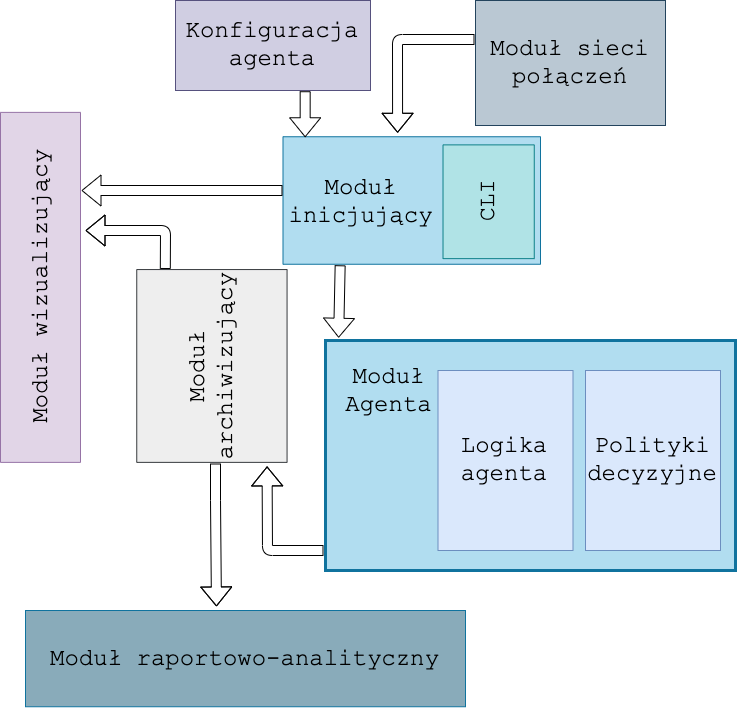
\includegraphics[width=\textwidth, height=0.7\textheight]{./png/system-arch.png}
	\caption{Architektura systemu z zaznaczanonymi modułami składowymi.}
	\label{arch1}
\end{figure}

\subsection{Moduł inicjujący}

Jest to moduł odpowiedzialny za inicjalizację wszystkich pozostałych składowych systemu oraz 
uruchomienie środowiska symulacji. Moduł ten:

\begin{itemize}

\item uruchamia moduł archiwizujący, w którym zapisywane są zdarzenia generowane przez agentów oraz stan systemu 
\item wczytuje z plików konfiguracyjnych strukturę połączeń między agentami oraz ich parametry wewnętrzne 
\item włącza interfejs graficzny pozwalający na komunikację z systemem za pomocą zbioru komend  
\item włącza moduł wizualizaujący sieć połączeń oraz zdarzenia, która zachodzą w trakcie symulacji.

\end{itemize}


\subsubsection{Sposób użycia}

W celu aktywacji modułu inicjalizującego, a tym samym całego systemu symulacyjnego należy użyć poniższej komendy 
\newline
\texttt{python run.py [-h] --config CONFIG [--log LOG] [--log\_stream {out,err}] [--vis VIS]}
\newline
w której należy podać:

\begin{itemize}
	\item ścieżkę do pliku z konfiguracją agentów \texttt{CONFIG}
	\item ścieżkę do pliku, w którym będzie zapisywane archiwum zdarzeń zaszłych w trakcie symulacji \texttt{LOG}
	\item strumień na który moduł archiwizujący będzie wypisał zdarzenia zaszłe w trakcie symulacji  
		\begin{itemize}
			\item \texttt{err}
			\item \texttt{out}
		\end{itemize}
	\item flagę aktywującą moduł wizualizacyjny \texttt{VIS}.
\end{itemize}
\subsection{Moduł sieci połączeń}
Moduł ten odpowiada za stworzenie sieci połączeń między agentami. Na rysunku (\ref{uml-net}) zawarty jest diagram 
klas UML przedstawiający metody dostarczane przez ten moduł.

\begin{figure}[H]
	\centering
	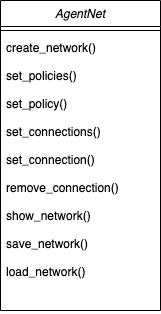
\includegraphics[width=0.3\textwidth, height=0.3\textheight]{./png/net-uml.png}
	\caption{Diagram klas modułu sieci połączeń.}
	\label{uml-net}
\end{figure}

Poza stworzeniem sieci połączeń moduł również ładuje polityki decyzyjne agentów oraz umożliwia zapis/odczyt sieci i jej parametrów
do/z plików \texttt{YAML}.


Moduł inicjujący odpowiedzialny jest również za aktywowanie interfejsu linii komend, w której użytkownik może komunikować się z systemem w trakcie trwania symulacji.
Dostępne możliwe komendy są następujące:

\begin{itemize}
	\item wyłączenie agenta z symulacji komendą o składni \texttt{kill [agent id]}
	\item ponowne włączenie agenta do symulacji komendą o składni \texttt{restore [agent id]}
	\item wyłączenie symulacji komedną \texttt{shutdown}.
\end{itemize}

W celu wprowadzania komend dedykowane jest specjalne okno, które widnieje na rysunku (\ref{run-image}) prezentującym działanie systemu.
\begin{figure}[H]
	\centering
	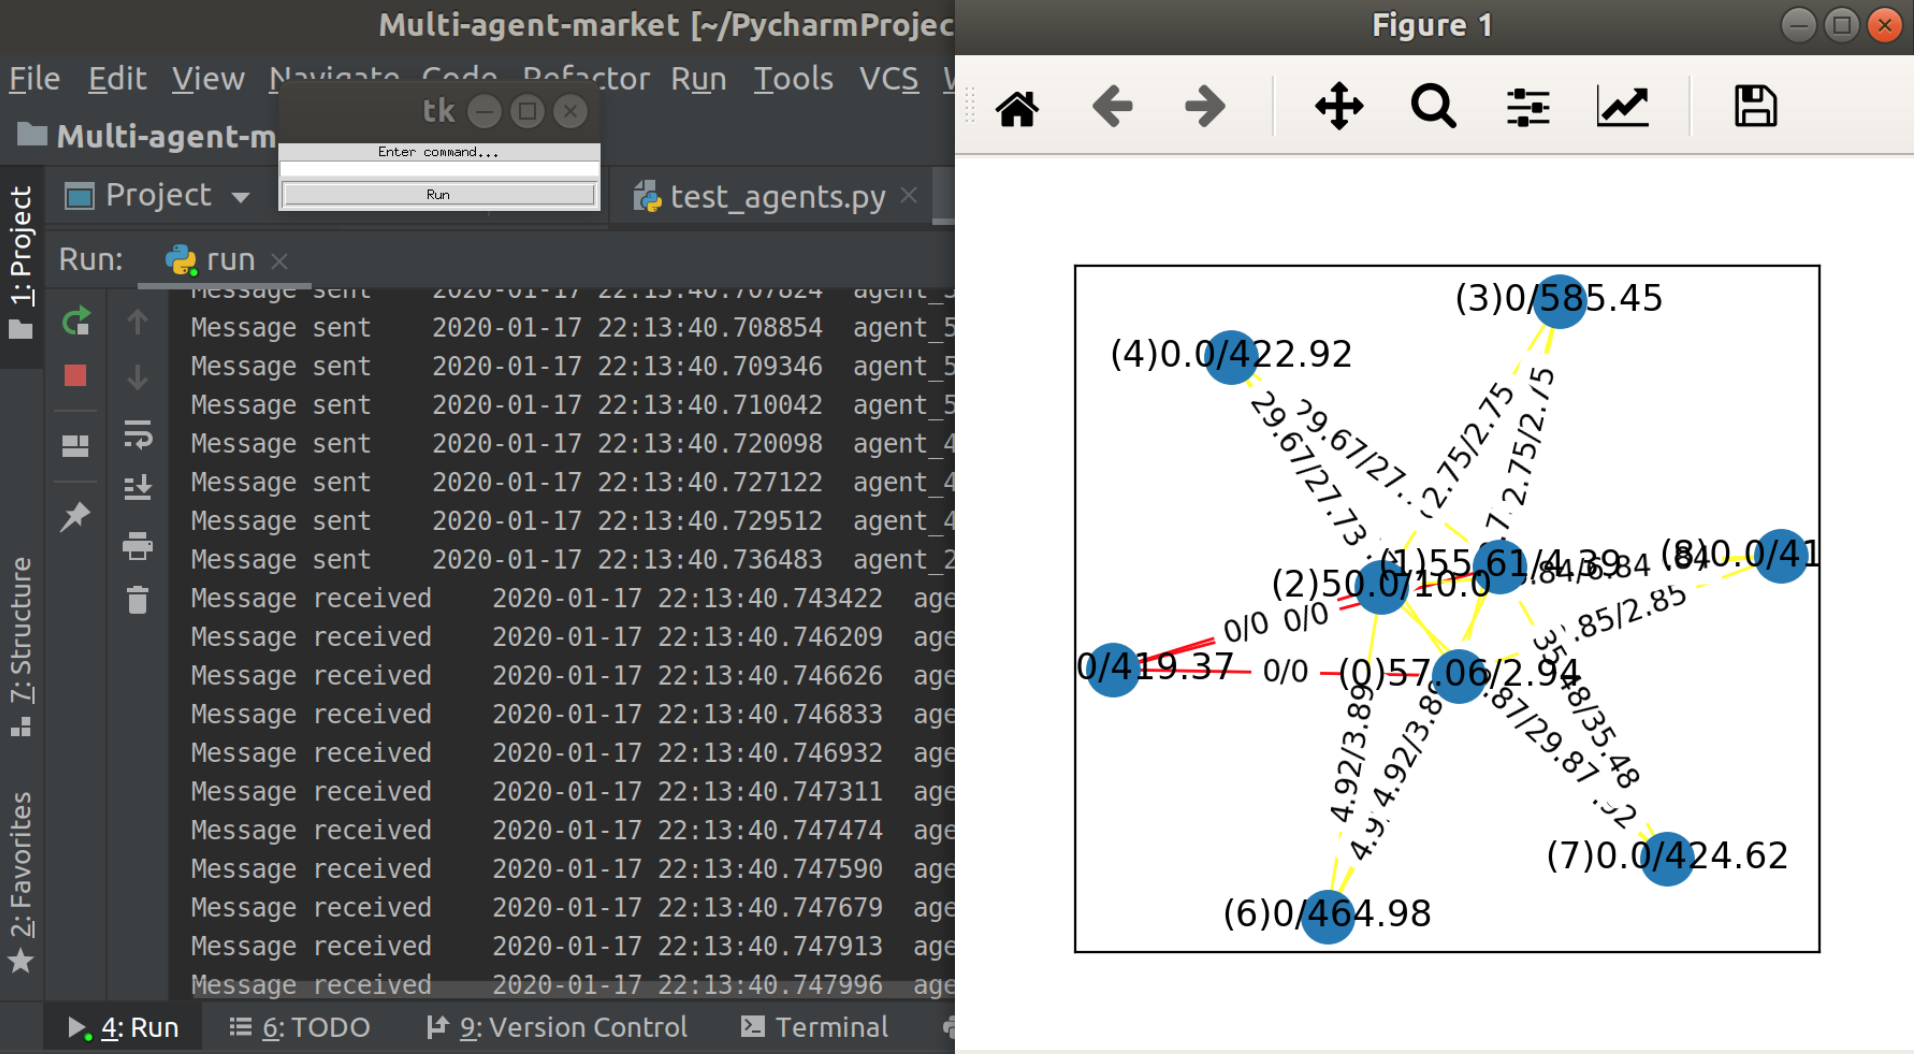
\includegraphics[width=\textwidth, height=0.5\textheight]{./png/run-image.png}
	\caption{System wypisuje archiwum zdarzeń na strumień standardowego wyjścia oraz widoczne jest działanie modułu wizualizaującego. Okno przy lewym górnym rogu zapewnia \texttt{CLI}.}
	\label{run-image}
\end{figure}


\subsection{Moduł konfiguracyjny}

Moduł konfiguracyjny odpowiedzialny jest za ustawienie wszystkich wartości parametrów agenta, które zostały  
opisane w sekcji (\ref{sec1}).
Na rysunku (\ref{uml-config}) zawarty jest diagram 
klas UML przedstawiający metody dostarczane przez ten moduł.

\begin{figure}[H]
	\centering
	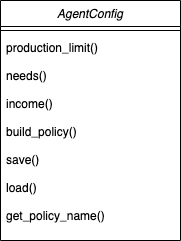
\includegraphics[width=0.3\textwidth, height=0.3\textheight]{./png/config-uml.png}
	\caption{Diagram klas modułu konfiguracyjnego.}
	\label{uml-config}
\end{figure}

Metody:
\begin{itemize}
	\item \texttt{production\_limit()}
	\item \texttt{needs()}
	\item \texttt{income()}
\end{itemize}

zwracają na podstawie aktualnego czasu symulacji oraz pewnego kroku czasowego $dt$ skalarną wartość odpowiedzialną za -- kolejno -- limit produkcji, potrzeby konsumpcyjne agenta
oraz przychód.

Pozostałe metody odpowiadają za wywołanie konstruktura polityk decyzyjnych oraz operacje zapisu/odczytu parametrów konfiguracyjnych z plików \texttt{YAML}.


\subsection{Moduł Agenta}

Moduł ten jest najbardziej złożonym elmentem systemu i składa się z dwóch podmodułów, które zostaną krótko scharakteryzowane:

\begin{itemize}
	\item modułu logiki agenta
	\item modułu polityk decyzyjnych agenta.
\end{itemize}


Na rysunku (\ref{uml-agent}) znajduje się diagram klas przedstawiający elementy składowe modułu agenta, tj.:

\begin{figure}[H]
	\centering
	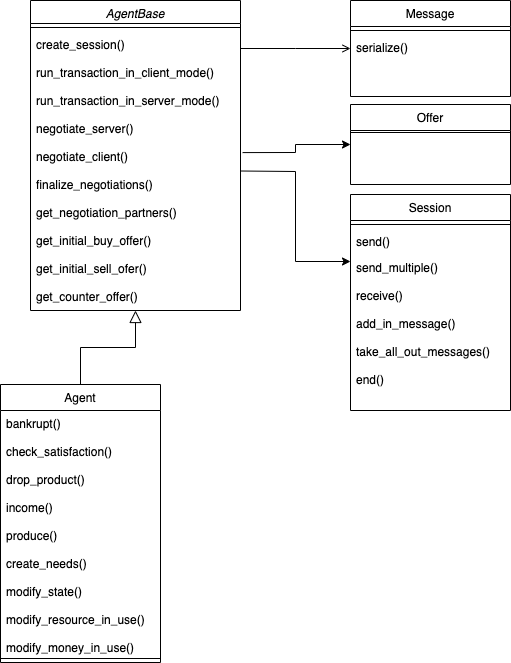
\includegraphics[width=0.8\textwidth, height=0.8\textheight]{./png/agent-uml.png}
	\caption{Diagram klas modułu agenta.}
	\label{uml-agent}
\end{figure}

\begin{itemize}
	\item klasę \texttt{AgentBase} implementującą model agenta zgodny z (\ref{sec1}) oraz zachowania agenta
		związane z generacją oraz wysyłaniem wiadomości
	\item klasę \texttt{Agent}, tj. klasę dziedziczącą po \texttt{AgentBase}, w której zaimplementowana jest logika 
		działania agenta
	\item klasę \texttt{Offer}, która reprezentuje ofertę formułowaną i nadawaną przez agenta
	\item klasę \texttt{Message}, która reprezentuje wiadomości wysyłane między agentami
	\item klasę \texttt{Session}, która modeluje sesję utrzymywaną przez agenta w ramach jego działania na rynku. 
\end{itemize}

\subsubsection{Logika agenta}

Logika agenta jest implementowana w klasie \texttt{Agent} i składają się na nią wszystkie możliwe akcje podejmowane przez agenta w trakcie trwania sesji. \\
Zbiór akcji agenta składa się z następujących elementów:

\begin{itemize}

	\item utworzenie oferty (klasa \texttt{CreateOffers})
	\item generacja produktu (klasa \texttt{GenerateProduct})
	\item usunięcie produktu (klasa \texttt{DropProduct}) 
	\item generacja potrzeb (klasa \texttt{ManageNeeds})
	\item generacja przychodu (klasa \texttt{GenerateIncome})
\end{itemize}

Wszystkie zachowania są modelowane jako zachowania cykliczne (\textit{CyclicBehaviour}) w sensie definiowanym przez bibliotekę \texttt{spade}.

\subsubsection{Polityki decyzyjne}

Podmoduł polityk decyzyjnych jest odpowiedzialny za przebieg wykonania akcji definiowanych w ramach logiki agenta.

Na rysunku (\ref{fig:uml-policy}) zawarty jest diagram 
klas UML przedstawiający metody dostarczane przez ten moduł.

\begin{figure}[H]
	\centering
	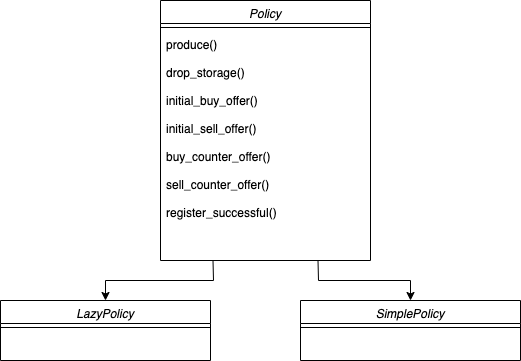
\includegraphics[width=0.8\textwidth, height=0.3\textheight]{./png/policy.png}
	\caption{Diagram polityk decyzyjnych.}
	\label{fig:uml-policy}
\end{figure}

Klasa \texttt{Policy} jest klasą abstrakcyjną po której dziedziczą klasy \texttt{LazyPolicy} oraz \texttt{SimplePolicy}.

Użytkownik posiada dowolność w definiowaniu klas polityk agentów z dokładnością do zgodności typów zwracanych przez funkcje.

\subsection{Moduł archiwizujący}

Moduł ten pozwala na wypisywanie informacji o stanie systemu na standardowe wyjście.
Na rysunku (\ref{uml-config}) zawarty jest diagram 
klas UML przedstawiający metody dostarczane przez ten moduł.

\begin{figure}[H]
	\centering
	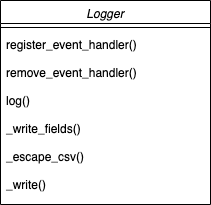
\includegraphics[width=0.3\textwidth, height=0.3\textheight]{./png/logger-uml.png}
	\caption{Diagram klas modułu archiwizującego.}
	\label{logger-agent}
\end{figure}

Umożliwia on także zapisywanie tych informacji do pliku. 
Na podstawie danych z tego modułu tworzona jest wizualizacja symulacji oraz część analityczna.
W tabeli (\ref{events-tab}) zawarte są wszystkie zdarzenia, które są przekazywane do modułu archwizującego. \\
Zdarzenia zostały podzielone na domeny, których dotyczą, tj.:

\begin{itemize}
	\item domena \textbf{Logger} dotyczy zdarzeń związanych z modułem archiwizującym
	\item domena \textbf{Agent} dotyczy zdarzeń związanych ze stanem agenta 
	\item domena \textbf{Sesja} dotyczy zdarzeń związanych z sesją handlową prowadzoną przez agenta 
	\item domena \textbf{System} dotyczy zdarzeń związanych z działaniem systemu 
\end{itemize}

\begin{table}[H]
	\begin{tabularx}{1.2\textwidth}{|X|X|}
\hline
\multicolumn{1}{|c|}{\textbf{Domena}} & \multicolumn{1}{c|}{\textbf{Zdarzenia}}                                                                                                                                                                                              \\ \hline
Logger                                & \small\textit{EVENT\_LOGGER\_INITIALIZED}                                                                                                                                                                                                  \\ \hline
Agent                                 & \small\textit{EVENT\_AGENT\_INITIAL\_OFFER, EVENT\_AGENT\_OFFER\_CHANGED, EVENT\_AGENT\_OFFER\_ACCEPTED, EVENT\_AGENT\_OFFER\_REJECTED, EVENT\_AGENT\_STATE\_CHANGED, EVENT\_AGENT\_BANKRUPTED} \\ \hline
Sesja                                 & \small\textit{EVENT\_MESSAGE\_SENT, EVENT\_MESSAGE\_RECEIVED, EVENT\_SERVER\_NEGOTIATION\_BREAKDOWN, EVENT\_CLIENT\_NEGOTIATION\_BREAKDOWN, EVENT\_SERVER\_FAILED\_TO\_RESPOND}               \\ \hline
System                                & \small\textit{EVENT\_SYSTEM\_INITIALIZED, EVENT\_SYSTEM\_CLOSE, EVENT\_EXCEPTION, EVENT\_CLI} \\ \hline
	\end{tabularx}
\caption{Tabela ze wszystkimi zdarzeniami, które odnotowuje moduł archiwizujący.}
\label{events-tab}
\end{table}

\subsection{Moduł wizualizujący}

Moduł ten pozwala na wyświetlanie symulacji w czasie rzeczywistym. \\

W węzłach grafu sieci połączeń przechowwany jest obecny stan agenta w formacie \texttt{liczba produktu/liczba środków wymiany}. 

Kolor krawędzi oznacza jaka akcja wykonywana jest w danym momencie przez agentów w ramach negocjacji handlowych: 

\begin{itemize}
    \item czarny -- bezczynny
    \item niebieski -- wysłanie oferty 
    \item żółty -- wysłanie kontroferty 
    \item czerwony -- zerwanie negocjacji
    \item zielony -- zaakceptowanie oferty 
\end{itemize}

Krawędzie opisane są liczbą produktu oraz środka wymiany, które są przedmiotem oferty w identycznym foramcie jak stan agenta w węźle. 

Na rysunku (\ref{vis-image}) zaprezentowana jest przykładowa wizualizacja symulacji.

\begin{figure}[H]
	\centering
	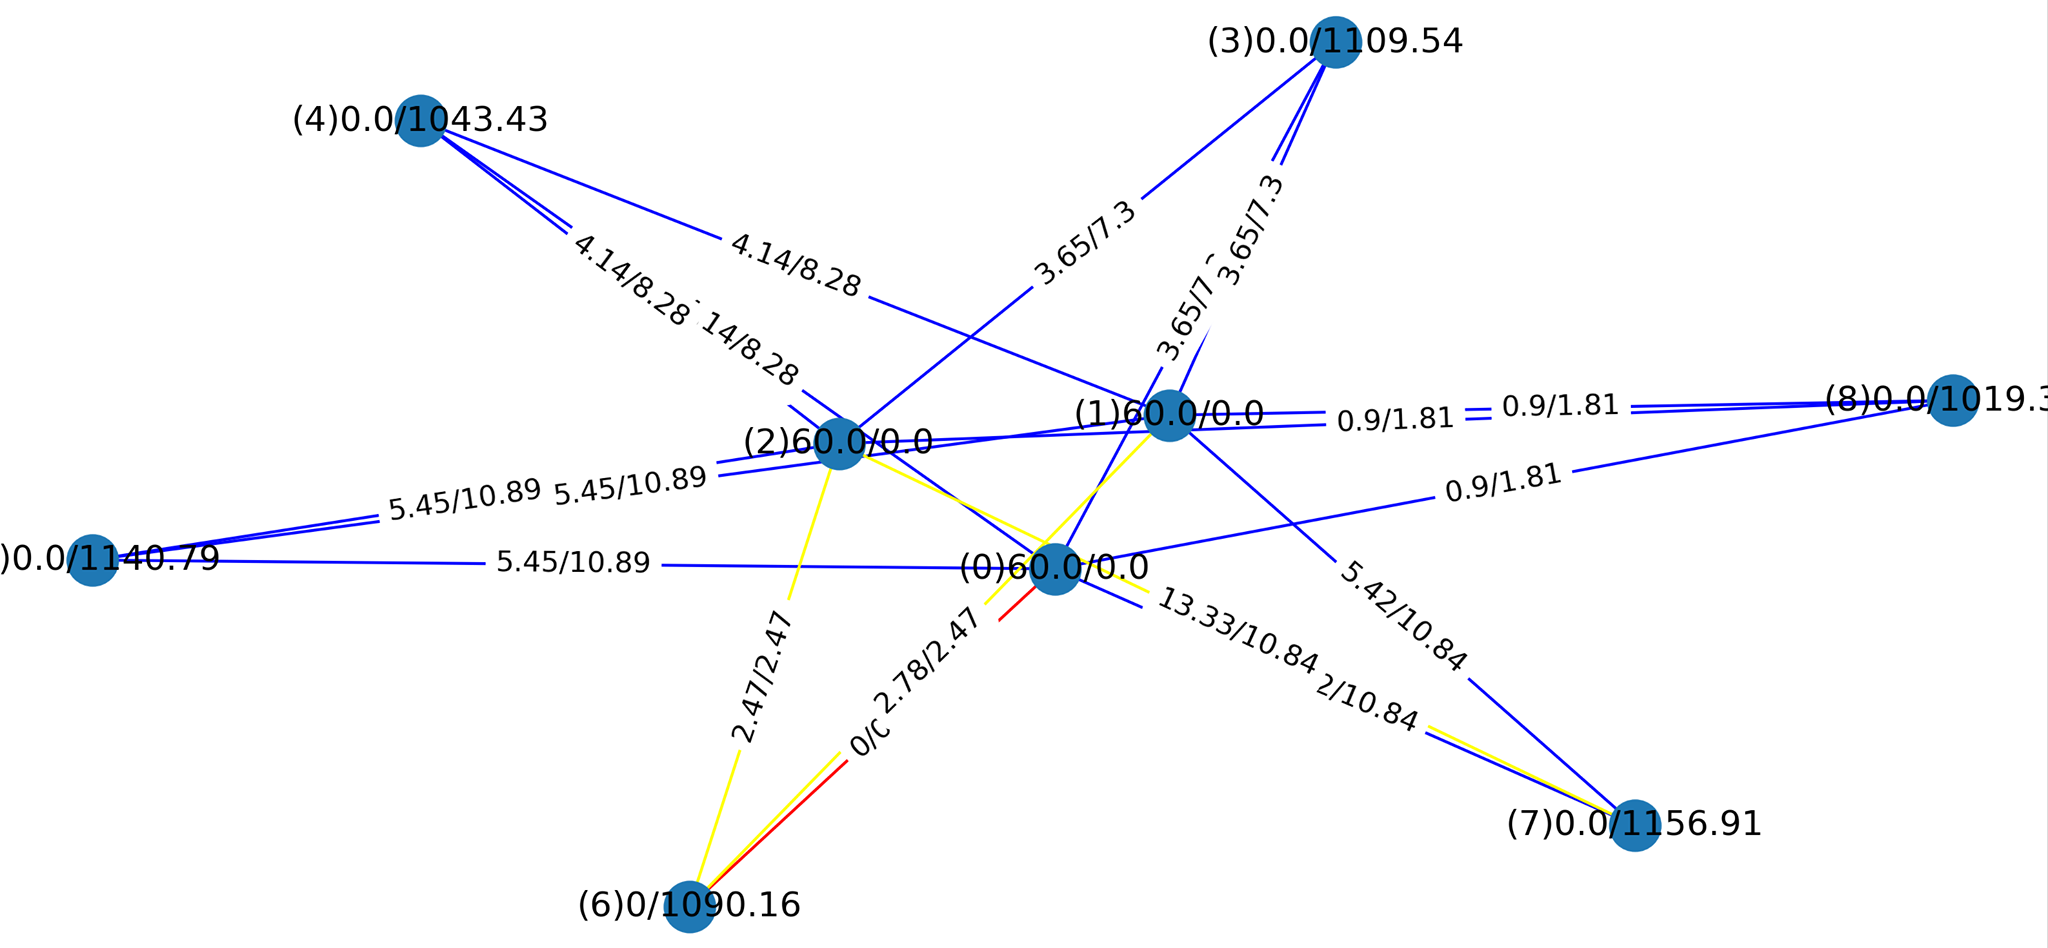
\includegraphics[width=\textwidth, height=0.4\textheight]{./png/vis-image.png}
	\caption{Wizualizacja symulacji złożonej z 9 agentów. Agent $(3)$ posiada 0 jednostek produktu oraz $1109.54$ jednostek środka wymiany.}
	\label{vis-image}
\end{figure}
\subsection{Moduł raportowo-analityczny}

Moduł ten składa się z szeregu funkcji napisanych w języku \texttt{R}, które na podstawie archiwum utworzonego w trakcie po przeprowadzeniu symulacji, pozwalają na:

\begin{itemize}
	\item ekstrakcje ustandaryzowanych ramek danych
	\item wizualizacji stanu agentów w czasie trwania symulacji, tj. ich liczby jednostek produktu oraz środka wymiany
	\item wizualizacji przebiegu ceny produktu w ramach ofert sprzedaży i kupna.
\end{itemize}

Przykładowy przebieg utworzony na podstawie archiwum symulacji znajduje się na rysunku (\ref{analytics-image}).


\begin{figure}[H]
	\centering
	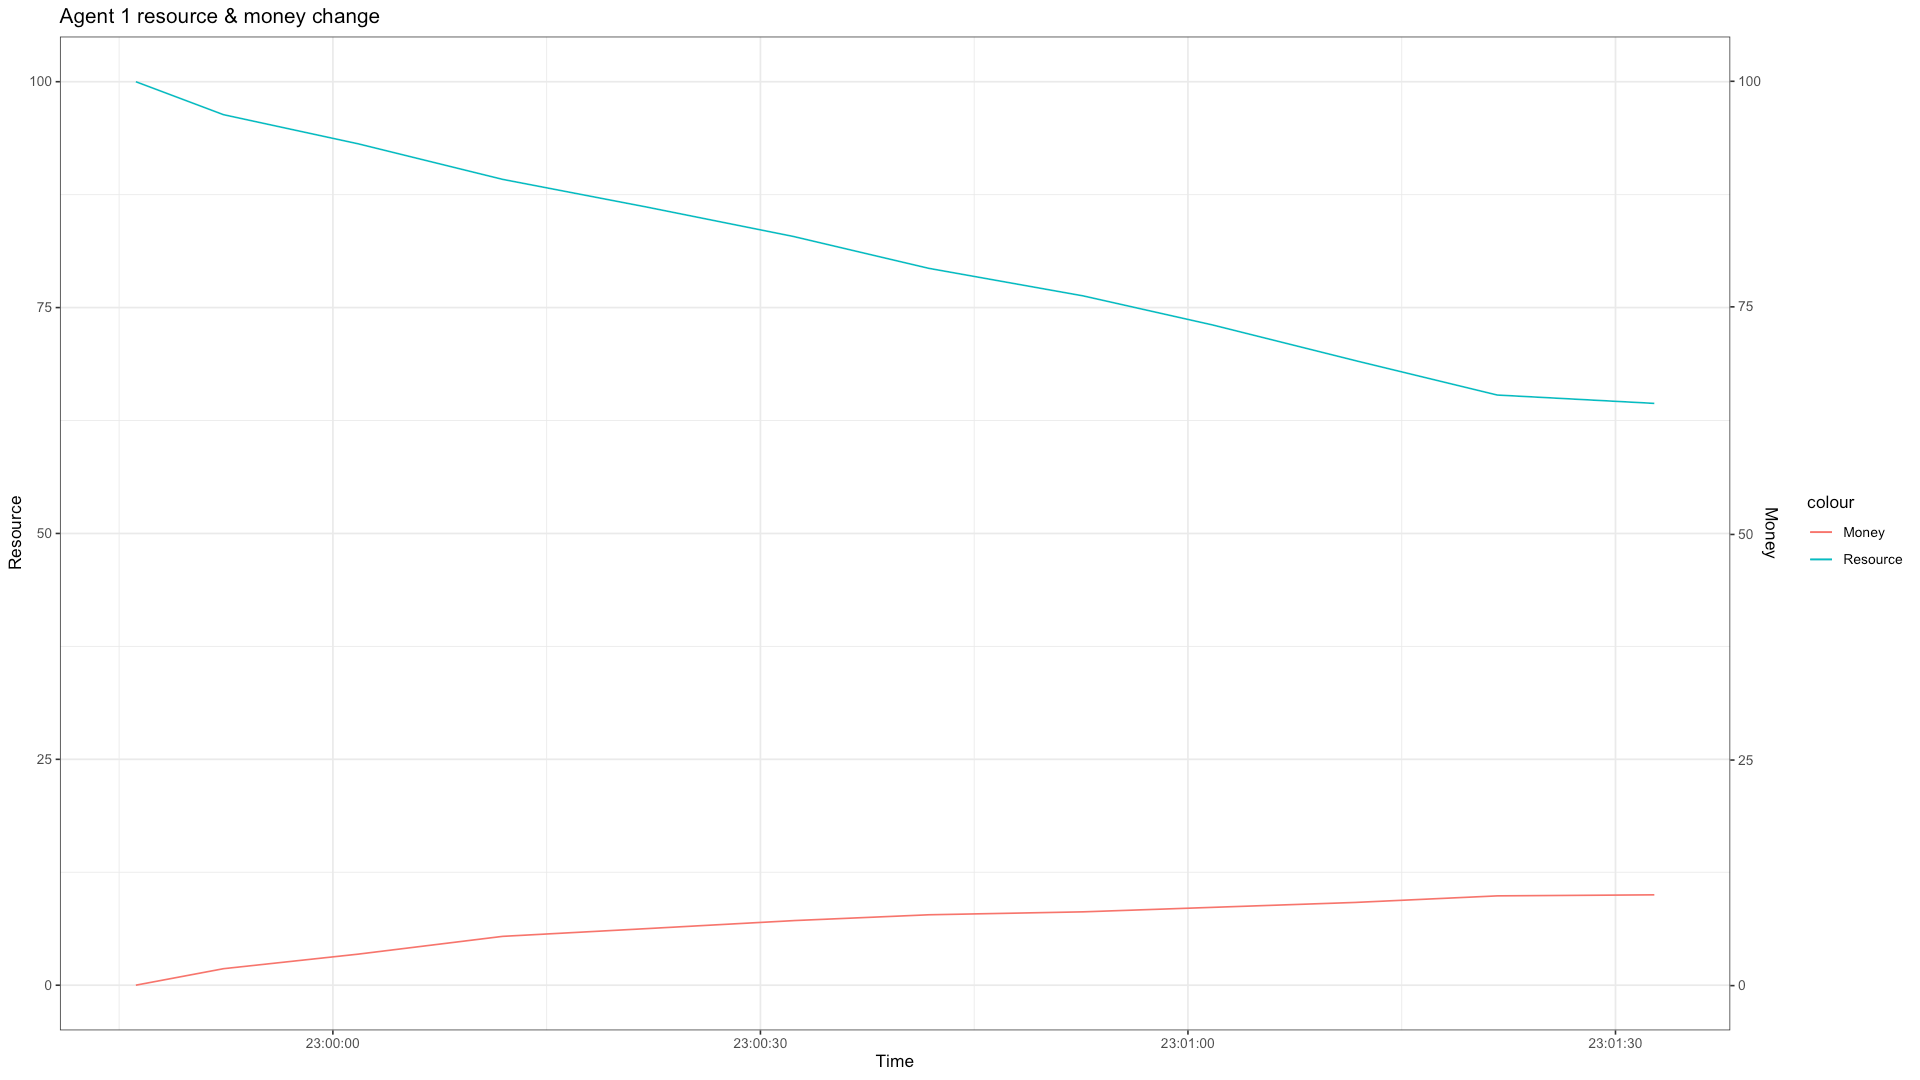
\includegraphics[width=\textwidth]{./png/analytics-image.png}
	\caption{Przebieg liczby posiadanych jednostek produktu oraz środków wymiany przez agenta.}
	\label{analytics-image}
\end{figure}

\section{Eksperymenty \label{sec3}}

W celu zaprezentowania możliwości zaprojektowanego i zaimplementowanego systemu w ramach projektu przeprowadzono trzy eksperymenty:

\begin{itemize}
	\item generacja monopolu, tj. eksperyment mający na celu zbadanie wpływu kosztu produkcji na możliwość utworzenia się monopolu na rynku dóbr konsumpcyjnych	
	\item działanie sieci wielkoskalowej, tj. eksperyment, w którym sprawdzano jak działa system w obliczu przeprowadzania symulacji dla wielu agentów oraz reakcje systemu na wyłączenie jednego z agentów
	\item odporność systemu na awarie, tj. eksperyment, w którym sprawdzono zachowanie systemu po wyłączeniu agenta ze zbioru agentów aktywnych oraz jego włączenia.
\end{itemize}


Ze względu na konieczną wiedzę ekspercką zakresu funkcjonowania rynków dóbr konsumpcyjnych i zachowań realnych agentów w tym środowisku -- 
poniższe eksperymenty mają jedynie charakter demonstracyjny.  

\subsection{Generacja monopolu}

W celu zbadania zjawiska generacji monopolu na rynku dóbr konsumpcyjnych wykorzystano konfigurację agentów, w której wyróżniono łącznie 4 agentów z czego dwóch sprzedających dobra oraz dwóch wyłącznie kupujących je. 
Jeden z agentów sprzedających dobra (agent o numerze ID \texttt{0}) posiadał ponadto bliska zera koszt produkcji, co było -- uproszczonym -- warunkiem powstania monopolu. \\
Sieć połączeń między agentami stanowiła graf pełny. Rysunek przedstawia (\ref{monopoly-resource}) przedstawia stan posiadania jednostek produktów, które przypadały na agenta. Na jego podstawie można zawaużyć, że negocjaje handlowe przebiegały głównie między agentem od numerze ID równym \texttt{0} oraz agentem o numerze ID równym \texttt{3}. Brak chęci udziału uczestniczenia w sesji handlowej pozostałych agentów wynikał z ustawienia parametrów ich polityk decyzyjnych oraz parametrów początkowych przy czym brak zaznaczonego przebiegu dla agentów o ID \texttt{1} oraz \texttt{2} oznacza samoistne wyłączenie się z sesji.

\begin{figure}[H]
	\centering
	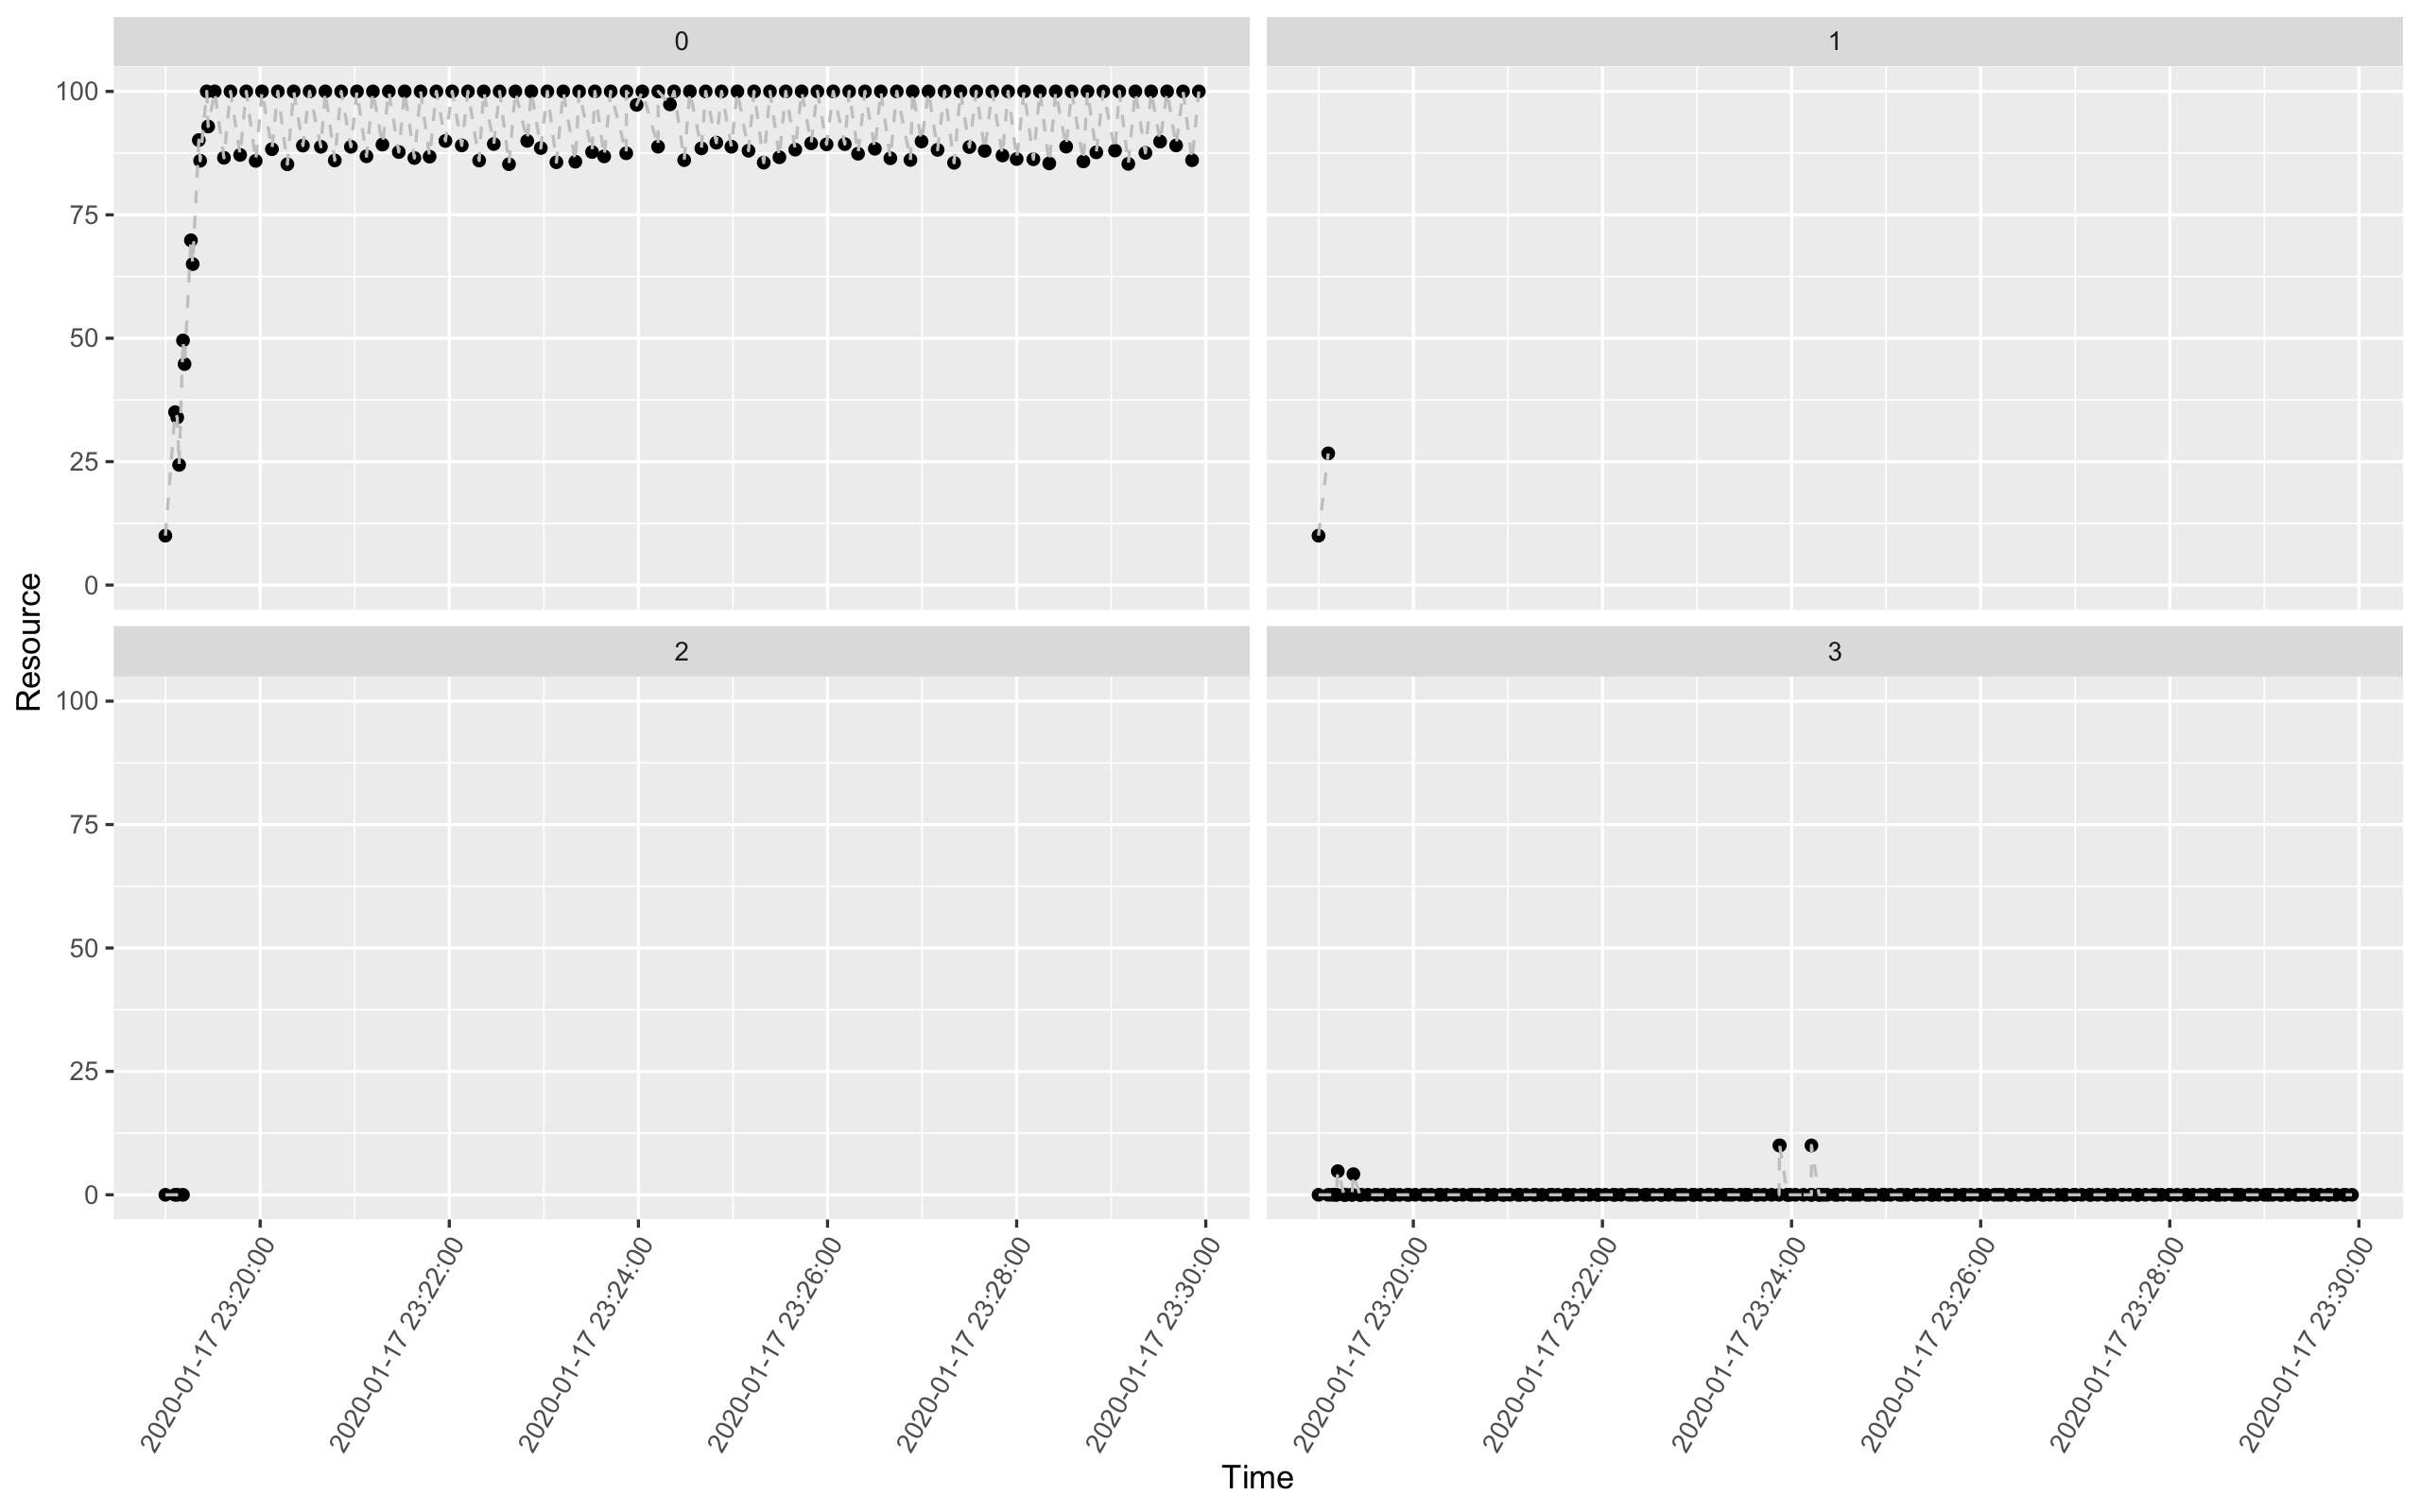
\includegraphics[width=\textwidth]{./png/monopoly-resource.png}
	\caption{Przebieg liczby posiadanych jednostek produktu przez agentów. Brak zaznaczonego przebiegu dla agentów o ID \texttt{1} oraz \texttt{2} oznacza samoistne wyłączenie się z sesji.}
	\label{monopoly-resource}
\end{figure}

Dominująca pozycja na rynku podmiotu o ID równym \texttt{0} ukazała się również w fakcie posiadanych przez niego jednostek środka wymiany, co obrazuje rysunek (\ref{monopoly-money})

\begin{figure}[H]
	\centering
	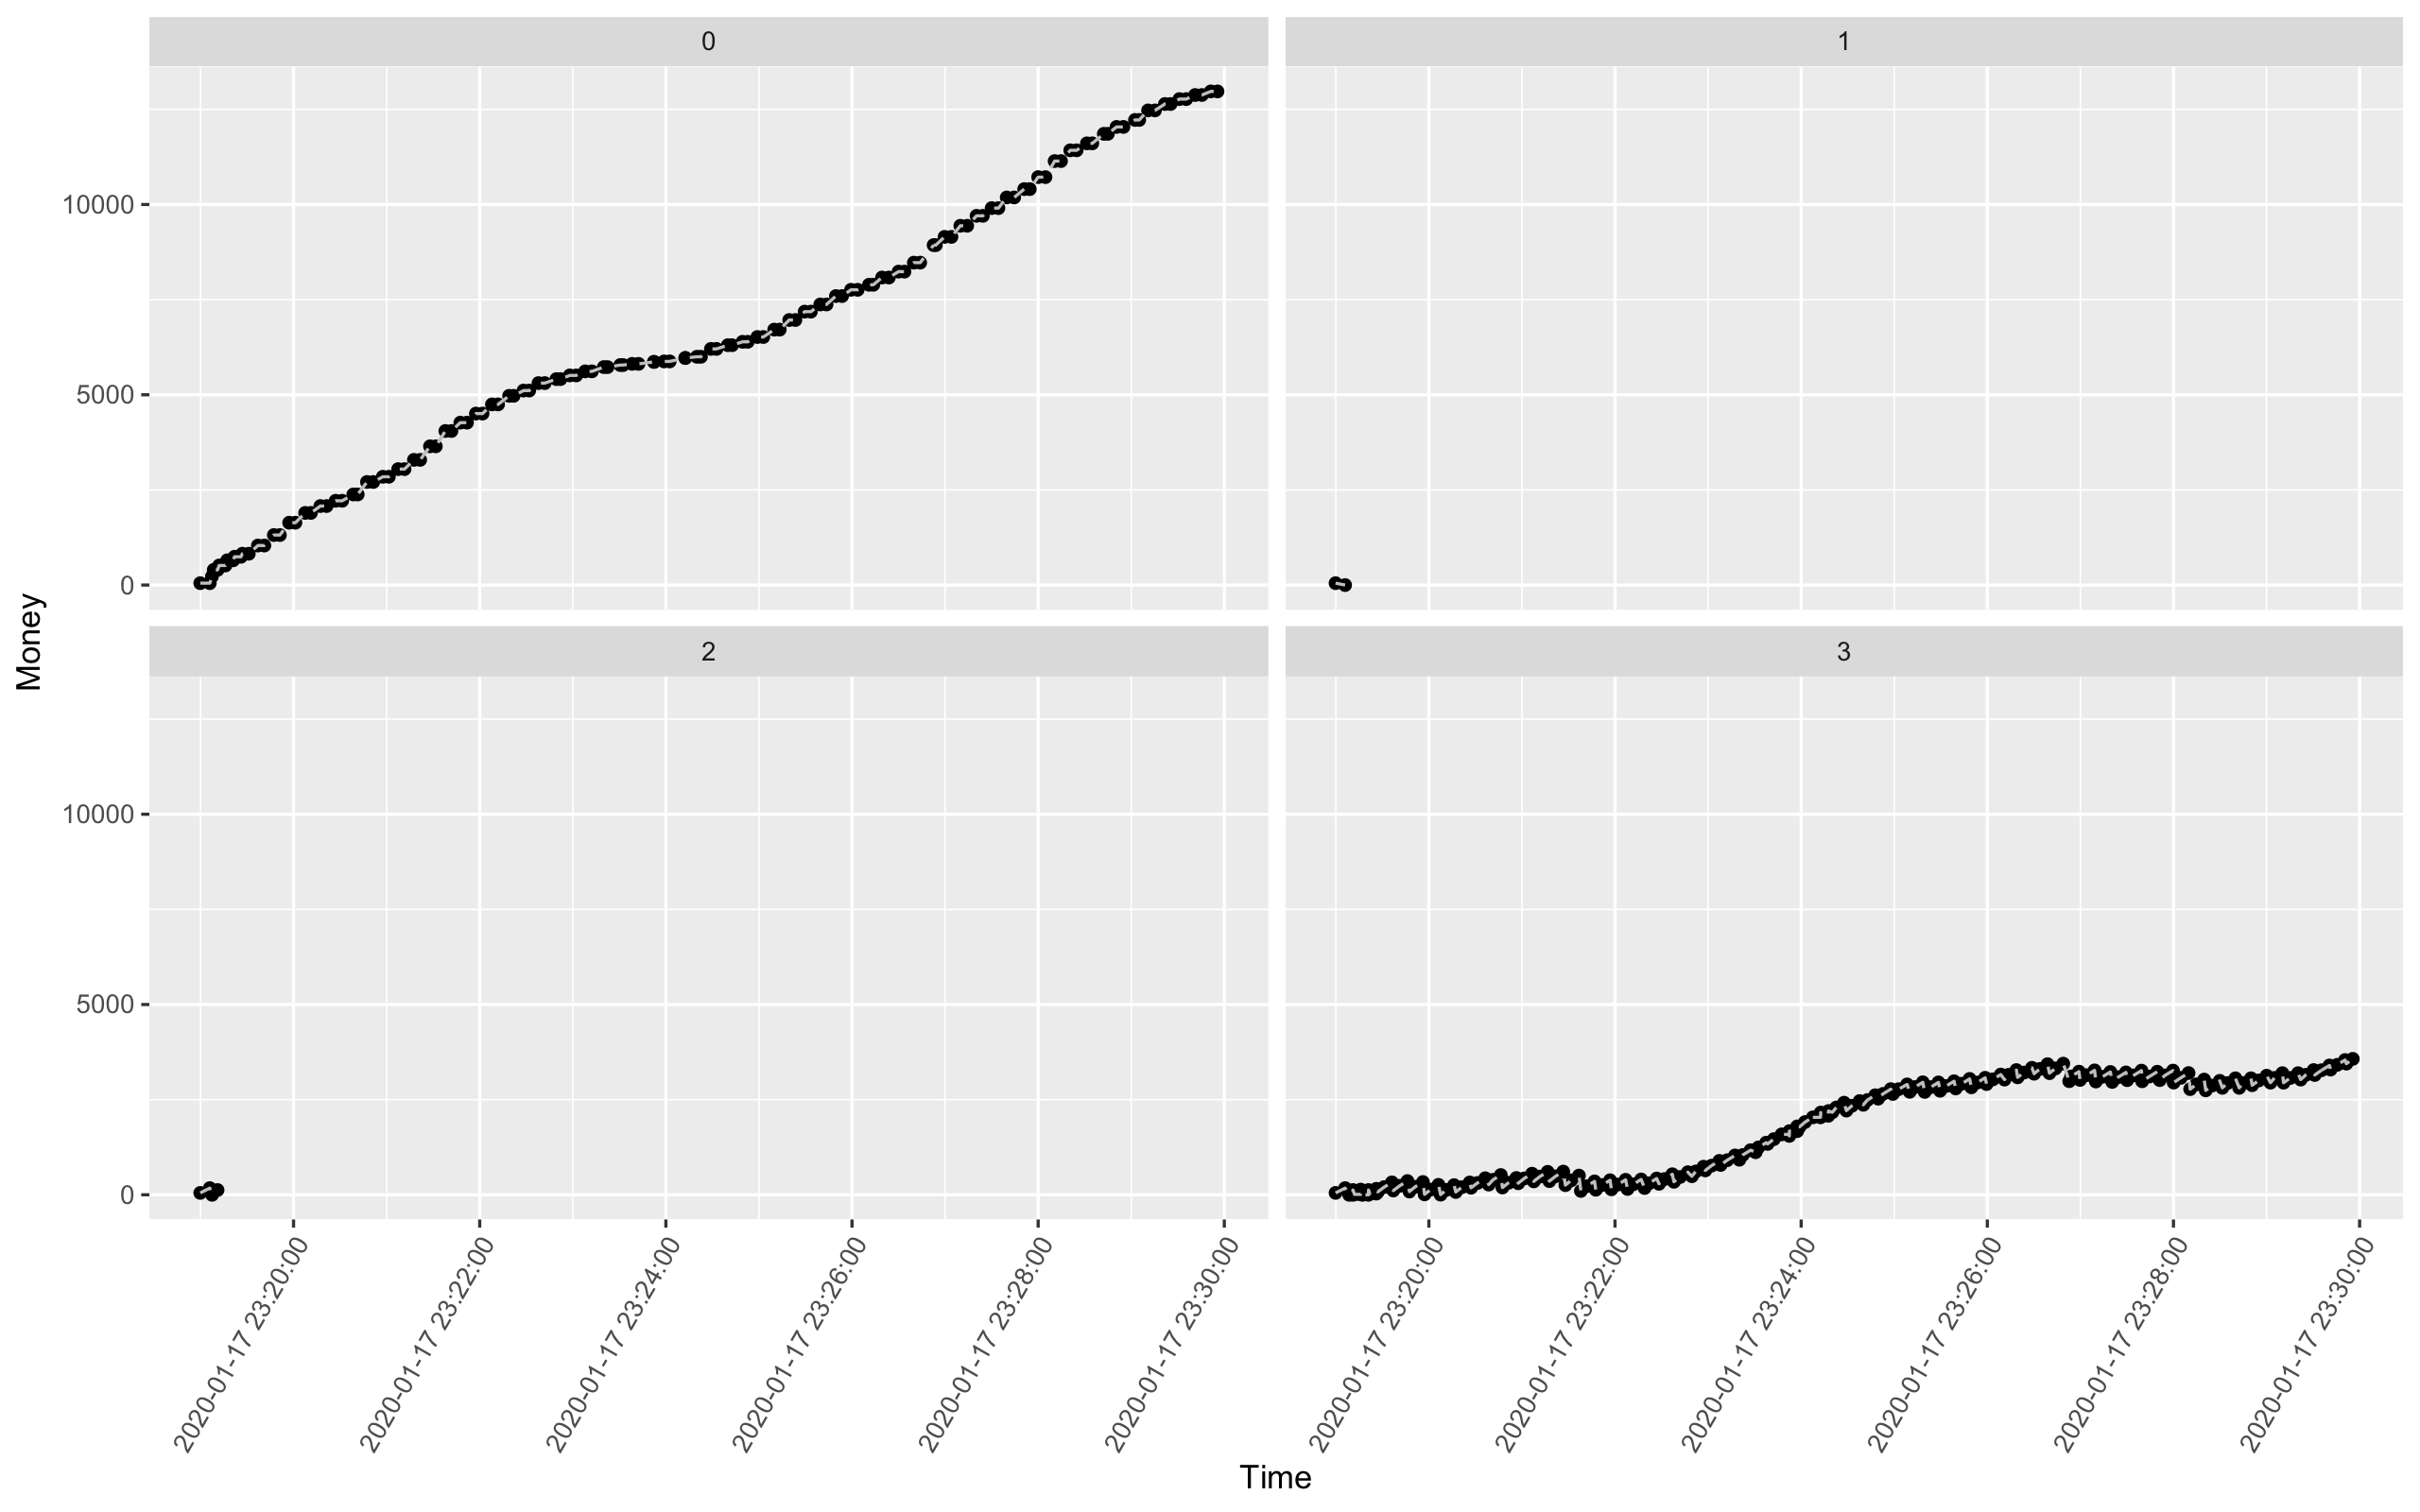
\includegraphics[width=\textwidth]{./png/monopoly-money.png}
	\caption{Przebieg liczby posiadanych środków wymiany przez agentów}
	\label{monopoly-money}
\end{figure}

\subsection{Działanie sieci wielkoskalowej \label{big-net}}

W ramach eksperymentów na systemie sprawdzono również w jaki sposób działa on, gdy liczba agentów jest duża -- w przypadku przyjętej konfiguracji było to dziewięciu agentów.
Sieć połączeń między nimi jest tożsama z siecią połączeń przedstawioną na rysunku (\ref{vis-image}).\\
Rysunek (\ref{big-net-money}) przedstawia zmianę cen produktu w ramach ofert sprzedaży oraz kupna. Ze względu na dużą liczbę agentów, a tym samym bardzo dużą liczbę zdarzeń na rynku cena podlegała częstym zmianom, co zauważalne 
jest po zagęszczeniu punktów na obu wykresach.

\begin{figure}[H]
	\centering
	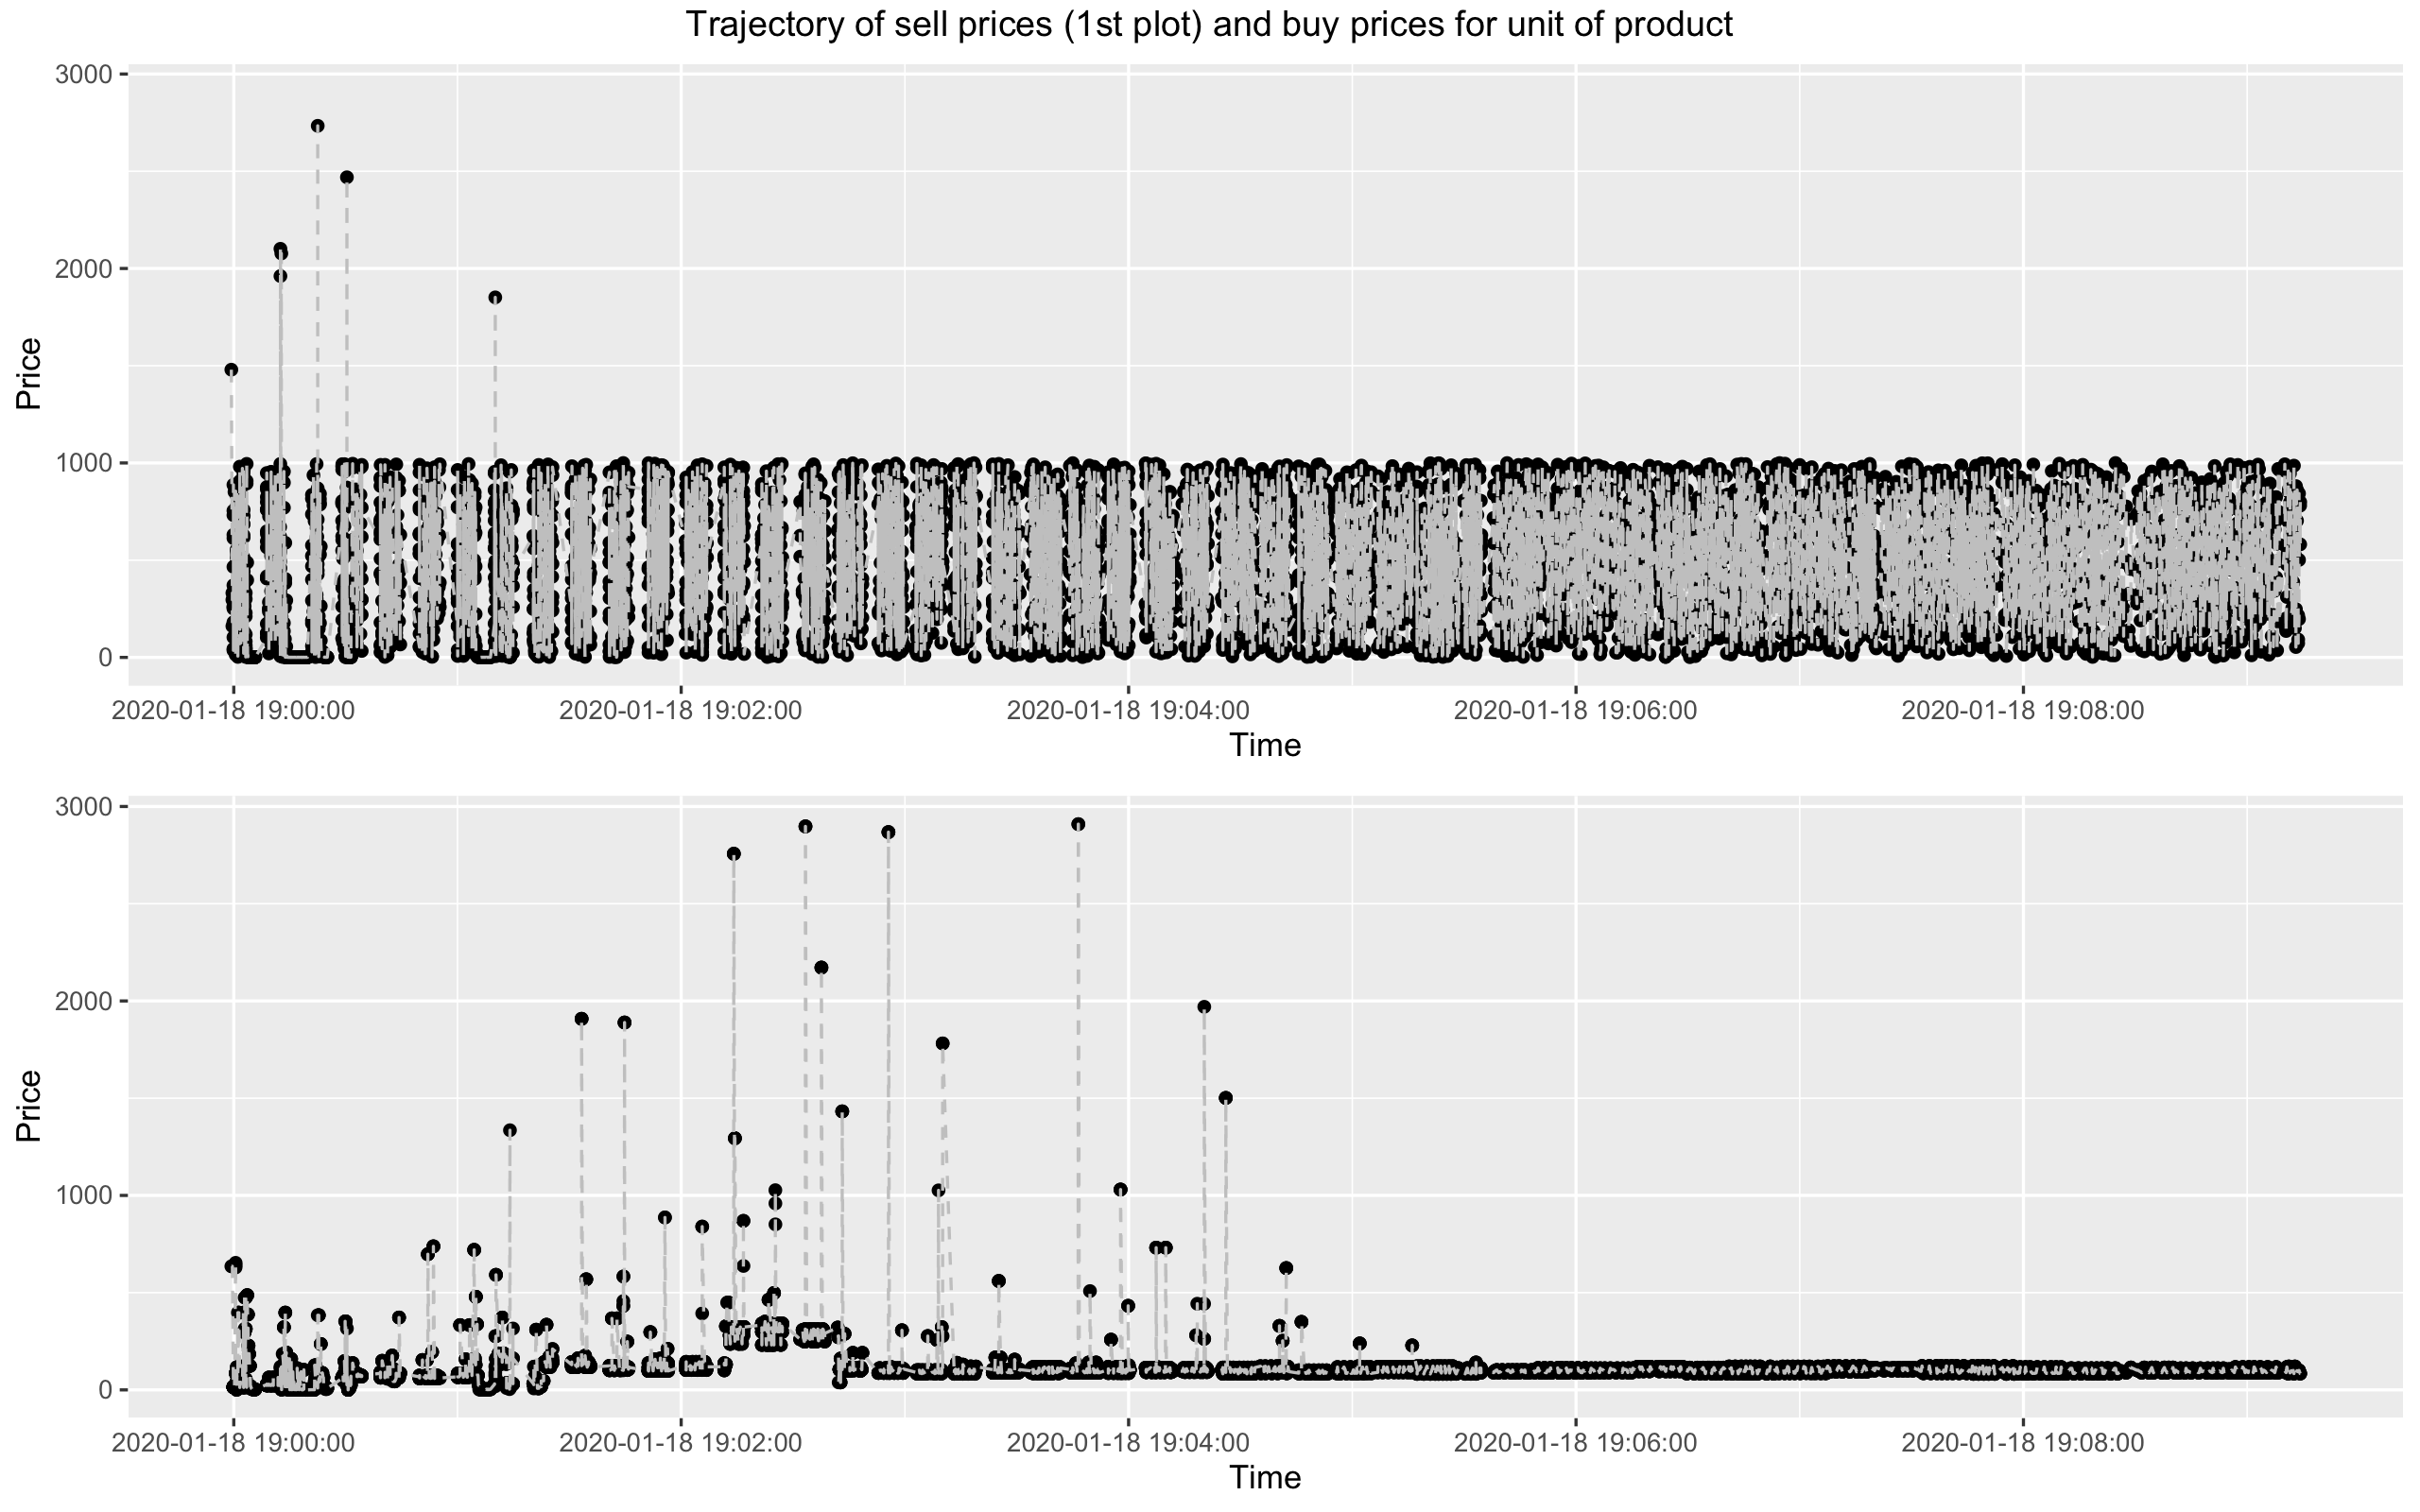
\includegraphics[width=\textwidth]{./png/big-net-money.png}
	\caption{Przebieg liczby posiadanych środków wymiany przez agentów}
	\label{big-net-money}
\end{figure}

\subsection{Odporność systemu na awarie}

W celu zbadania odporności systemu na awarie zbadano jego zachowanie w obliczu wyłączenia jednego z agentów. W związku z faktem, że na infrastrukturę systemu składają się wyłącznie agenty i to na podstawie ich stanu generowana 
jest sieć połączeń lub przebieg symulacji, przeprowadzenie takiego eksperymentu i przeanalizowanie jego wyników powinno zwrócić kompletną informację o t.zw. \textit{fault-tolerant} zaimplementowanego systemu. \\

Warunki początkowe eksperymentu są równoważne warunkom z eksperymentu opisanego w sekcji (\ref{big-net}). 
W trakcie jego trwania przy pomocy dostarczanej linii komend wyłączono agenta o ID równym $7$, co zostało odnotowane przez moduł archiwizujący i jest widoczne na rysunku (\ref{killed}). Ponadto widoczne jest tam, że agenty
dalej podejmują dostępne akcje z tą różnicą, że z ich sieci połączeń wyłączony jest agent o ID równym $7$.

\begin{figure}[H]
	\centering
	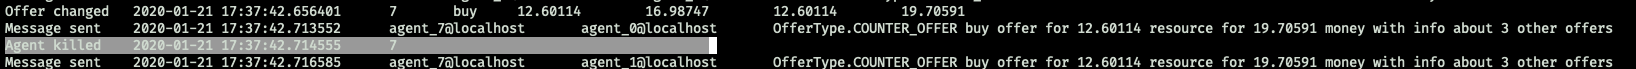
\includegraphics[width=\textwidth]{./png/killed.png}
	\caption{System poprawnie odnotowuje wyłączenie jednego z agentów.}
	\label{killed}
\end{figure}

Po pewnej chwili wyłączony wcześniej agent został przywrócony, co jest widoczne na rysunku (\ref{restarted}).

\begin{figure}[H]
	\centering
	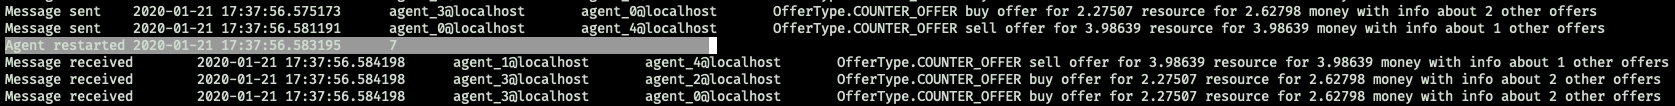
\includegraphics[width=\textwidth]{./png/restared.png}
	\caption{System poprawnie odnotowuje przywrócenie jednego z agentów.}
	\label{restared}
\end{figure}

Przywrócenie agenta spowodowało, że ponownie zaczął on brać udział w transakcjach handlowych, co można zauważyć na rysunku (\ref{offers}). 

\begin{figure}[H]
	\centering
	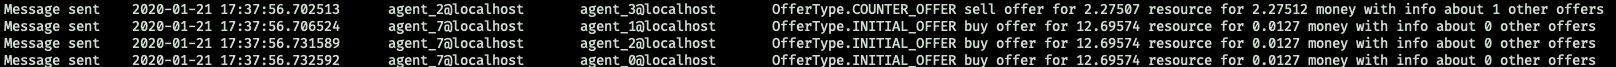
\includegraphics[width=\textwidth]{./png/offers.png}
	\caption{Przywrócony agent formułuje oferty handlowe.}
	\label{offers}
\end{figure}

Ponadto pozostałe agenty w systemie poprawnie reagują na jego oferty handlowe, co świadczy o poprawnym włączeniu uprzednio wyłączonego agenta do ich sieci połączeń (patrz rys. \ref{reactions}).


\begin{figure}[H]
	\centering
	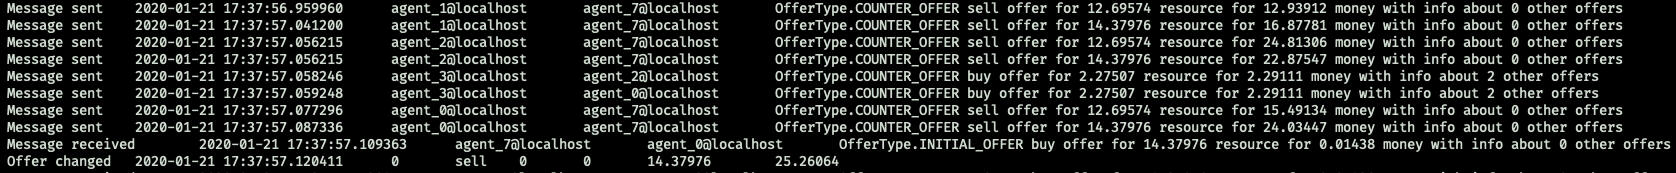
\includegraphics[width=\textwidth]{./png/reactions.png}
	\caption{Pozostałe agenty poprawnie reagują na obecność przywróconego agenta.}
	\label{reactions}
\end{figure}



\end{document}


